%!TEX root=../robocert.tex
\begin{figure}
	\centering
	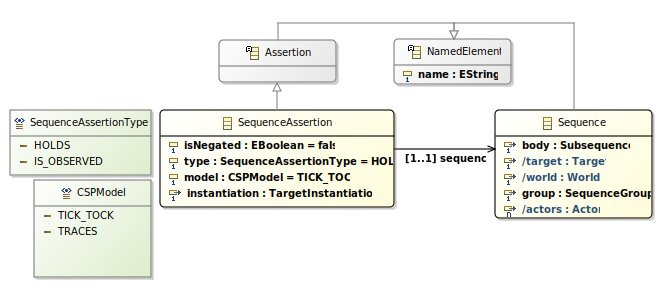
\includegraphics[width=0.7\textwidth]{diagrams/Assertions}
	\caption{Class diagram for the part of the \langname{} metamodel dealing with assertions.}
	\label{fig:metamodel-assertions}
\end{figure}

\Cref{fig:metamodel-assertions} depicts the part of the metamodel concerning
assertions.

\subsection{\massertion}

An \massertion{} is a named assertion statement.  Currently, there is
only one type of assertion: a \msequenceassertion{}.  \todo{This will change
when merging with the existing language, if not sooner.}

\subsection{\msequenceassertion}\label{ssec:metamodel-assertions-sequence}

A \msequenceassertion{} is an assertion about a particular \msequence{} with
respect to its \mtarget.  The \mtarget{} is modified by applying an
assertion-level \mtargetinstantiation, which may fix any constants not bound
by the sequence-level instantiation.  (The default is an empty instantiation,
meaning the target is exactly as specified at the sequence level.)

The specific sequence assertion type comes from the \msequenceassertiontype:
either `sequence holds on target' (refinement), or `sequence is observed on
target' (reverse refinement).  The assertion can be negated.  The choice of
\mcspmodel{} affects how the assertion is checked with CSP tools such as FDR
\todo{the models aren't actually used yet; everything is treated as untimed
traces refinement.  This will change.}

\begin{lstlisting}[style=Example]
assertion A: SequenceName holds           // positive 'holds' SequenceAssertion
assertion B: SequenceName does not hold   // negative 'holds' SequenceAssertion
assertion C: SequenceName is observed     // positive 'is observed' SequenceAssertion
assertion D: SequenceName is not observed // negative 'is observed' SequenceAssertion

assertion E: SequenceName holds with { CONSTANT set to 5 }
// example of SequenceAssertion with custom TargetInstantiation
\end{lstlisting}

%%% Local Variables:
%%% mode: latex
%%% TeX-master: "../robocert"
%%% End:
